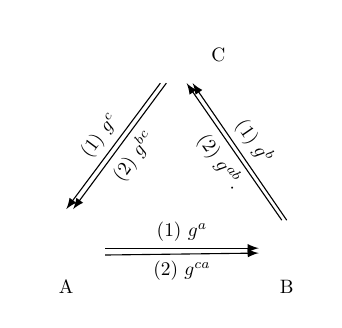
\begin{tikzpicture}[scale=0.7, every node/.style={scale=0.7}]
\node (A) at (0,0) [minimum size=1.4cm] {}; \Alice{0}{0}{0.4};
\node [below of = A, node distance = 0.7cm] {A};
\node (B) [right of = A, node distance = 4cm, minimum size=1cm] {}; \Bob{4cm}{0}{0.4};
\node [below of = B, node distance = 0.7cm] {B};
\node (C) at (2,3.5) [rounded corners=1ex,minimum size=1cm,label distance=-1cm,label=right:C] {};
\Charlie{2}{3.5}{0.4};
\draw[-latex] (A) -- (B) node [midway,above] {(1) $g^a$};
\draw[-latex] (A.350) -- (B.190) node [midway,below] {(2) $g^{ca}$};
\draw[-latex] (C.240) -- (A.90)  node [sloped,midway,above] {(1) $g^c$};
\draw[-latex] (C.250) -- (A.80)  node [sloped,midway,below] {(2) $g^{bc}$};
\draw[-latex] (B.90) -- (C.300) node [sloped,midway,above] {(1) $g^b$};
\draw[-latex] (B.100) -- (C.290) node [sloped,midway,below] {(2) $g^{ab}$.};
\end{tikzpicture}